\section{Results and Analysis}
	Using the test setup and cases shown above, we were able to gain the following insights.
	\subsection{DSSS}
		\subsubsection{Performance in presence of narrowband and wideband interference}~\\
			Figure \ref{fig:dsss_narrowband} shows error rates of DSSS under the influence of narrowband noise. We observe that higher \emph{chipping rates} - which lead to broader spreading - add robustness.
			This is due to the narrowband interference getting despread more strongly when employing higher chipping rates.
			The \emph{chip sequence length} has little to no influence, which also matches our expectations, as the power spectrum does not change with different chip length. Longer chip sequences do, hovewer, add support for more users.
			
			Figure \ref{fig:dsss_wideband} illustrates behaviour under the influence of wideband noise, which is nearly identical for all our different testing parameters.
			We would intuitively have expected low \emph{chipping rates} to have better performance - due to their more narrow frequency spectrum and thus higher peak power - but this line of thought ignores that wideband noise is not correllated with the sent signal, and so does not get despread. Thus, it remains on the same power level after despreading, which results in the invariability of performance under changing parameters.
			
			Due to our testing setup and methodology, direct comparison between the two scenarios is tedious. As our jammer implementation puts out a constant base power when measured over the whole spectrum, the SNRs tend to vary a lot for different scenarios. Because of that, we have chosen to regard narrowband and wideband noise as separate cases and do a comparison in a separate test case, where we tried to visually match the signal and noise spectra of the scenarios outlined in \cite{ISS}. The results of that test are shown in \ref{fig:dsss_bandwidth} and discussed in the next section.
				\begin{figure}[H]
					\centering
					\caption{}
				    \begin{subfigure}[b]{0.5\textwidth}
						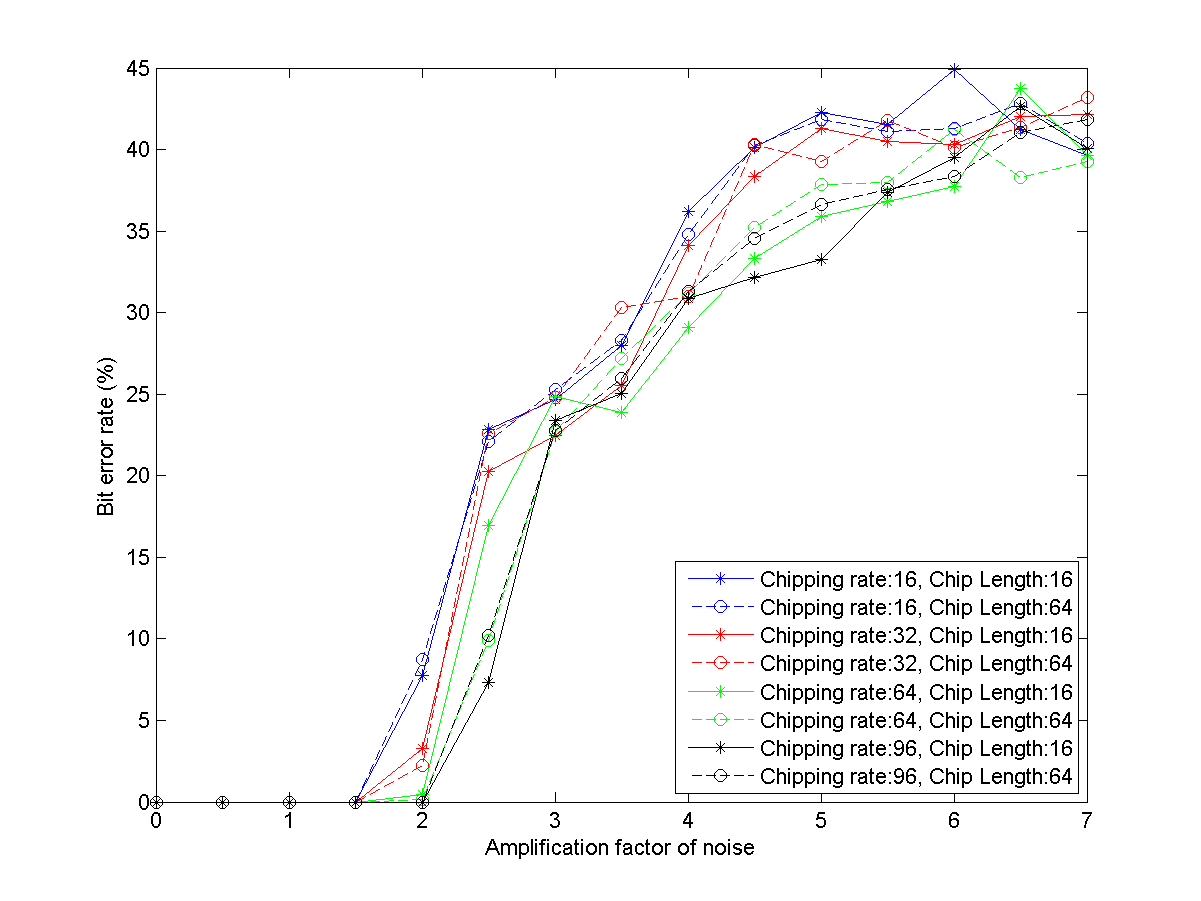
\includegraphics[width=\textwidth]{imgs/results/plot_mode_dsss-test_narrowband-rep_20-dataRate_8-dataLength_128.png}
						\caption{DSSS Narrowband noise: $\Delta f= 8 \text{Hz}, f_{jam} = 100\text{Hz}$}
						\label{fig:dsss_narrowband}
					\end{subfigure}%
					~
					\begin{subfigure}[b]{0.5\textwidth}
						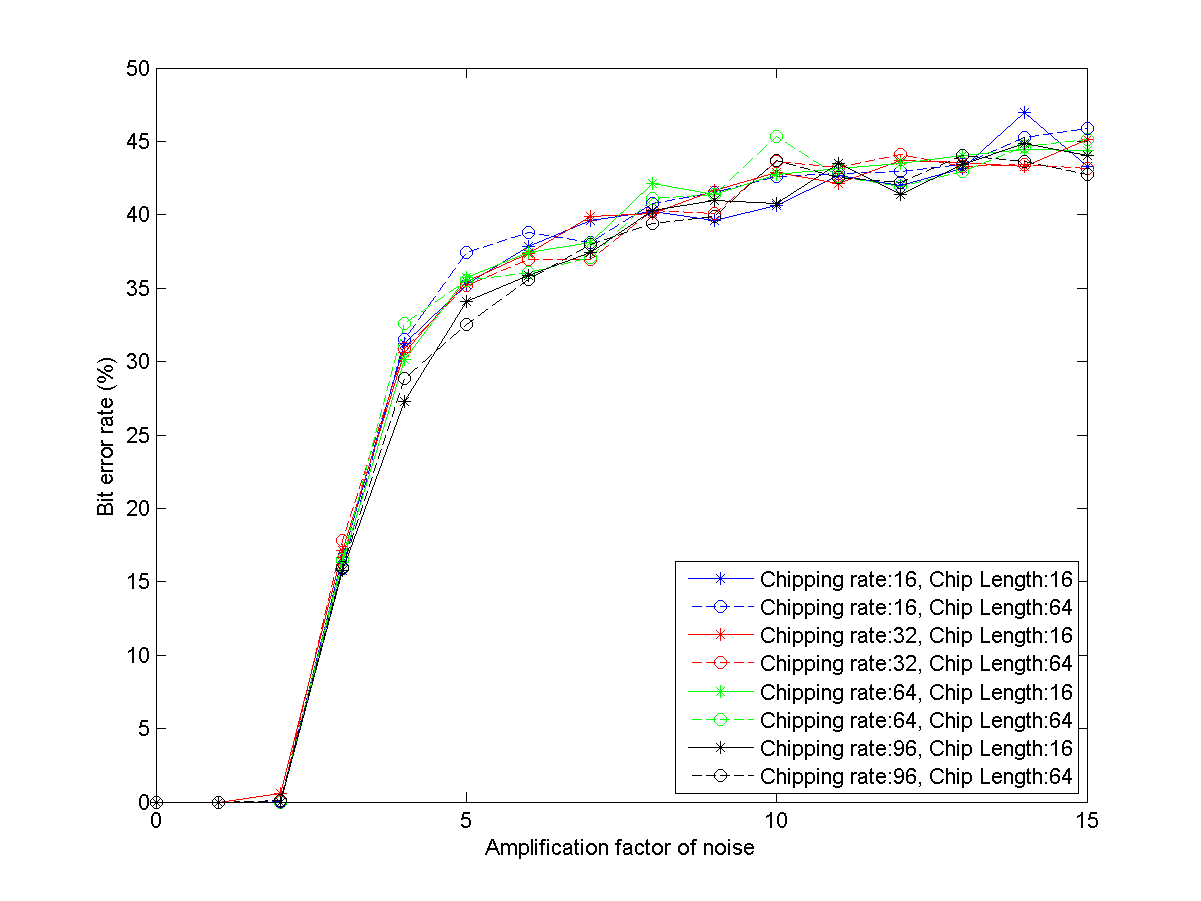
\includegraphics[width=\textwidth]{imgs/results/plot_mode_dsss-test_wideband-rep_20-dataRate_8-dataLength_128.png}
						\caption{DSSS Wideband noise: $\Delta f = 200 \text{Hz}, f_{jam} = 100\text{Hz}$}
						\label{fig:dsss_wideband}
					\end{subfigure}
				\end{figure}
				
		
		\subsubsection{Performance with varying interference bandwidth and white Gaussian noise}\label{sec:real-life}~\\
			Figure \ref{fig:dsss_bandwidth} shows the results of the aforementioned test case.
			\emph{Wideband noise} has a bigger impact on performance than \emph{narrowband noise} with high \emph{chipping rates} showing better performance than low ones.
			While we are very aware that the parameters for this configuration may seem arbitrary, we struggled to find reliable reference values. The result of this is that the results should be seen as a qualitative estimation of real-world performance of DSSS under presumably realistic levels and bandwidths of interference and not as exact values. 
			
			Figure \ref{fig:dsss_gaussian} outlines performance of our DSSS implementation with varying levels of white Gaussian noise.
			The results widely match expected behaviour, with performance deteriorating with more added noise.
			Unexpectedly, performance was worse when employing low chipping rates.
			We suspect this may be due to the way MATLAB measures the SNR when using the \emph{awgn} function.
			
			\begin{figure}[H]
				\centering
				\caption{}
				\begin{subfigure}[b]{0.5\textwidth}
					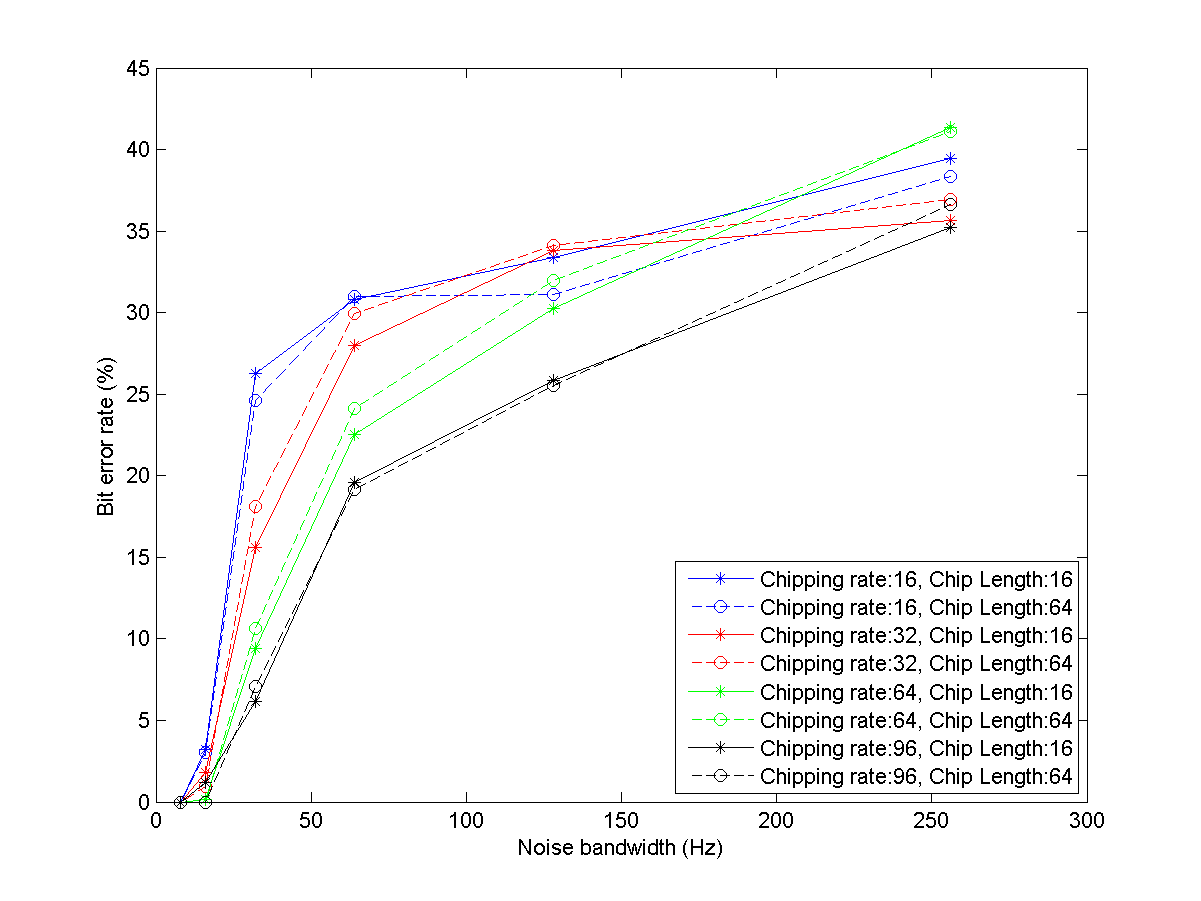
\includegraphics[width=\textwidth]{imgs/results/plot_mode_dsss-test_bandwidthAndPower-rep_20-dataRate_8-dataLength_128.png}
					\caption{DSSS: Various noise bandwidths and powers: $p_f = (1,2,2.5,3,3.5,4)$}
					\label{fig:dsss_bandwidth}
				\end{subfigure}%
				~
				\begin{subfigure}[b]{0.5\textwidth}
					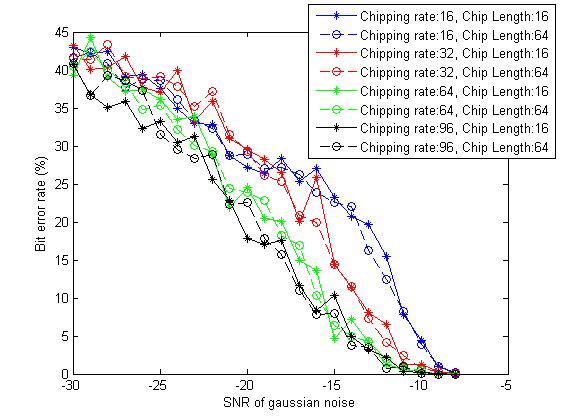
\includegraphics[width=\textwidth]{imgs/results/plot_mode_dsss-test_gaussianSNR-rep_20-dataRate_8-dataLength_128_fixedlegend.png}
					\caption{DSSS: Various SNR of white Gaussian noise}
					\label{fig:dsss_gaussian}
				\end{subfigure}
			\end{figure}		
				
		\subsubsection{Performance with multiple users}~\\
				
			In Figure \ref{fig:dsss_multiuser} we see that low \emph{chipping rates} work considerably worse than high chipping rates, as the signal is spread less.
			This matches expected behaviour.
				
			\begin{figure}[H]
			\centering
				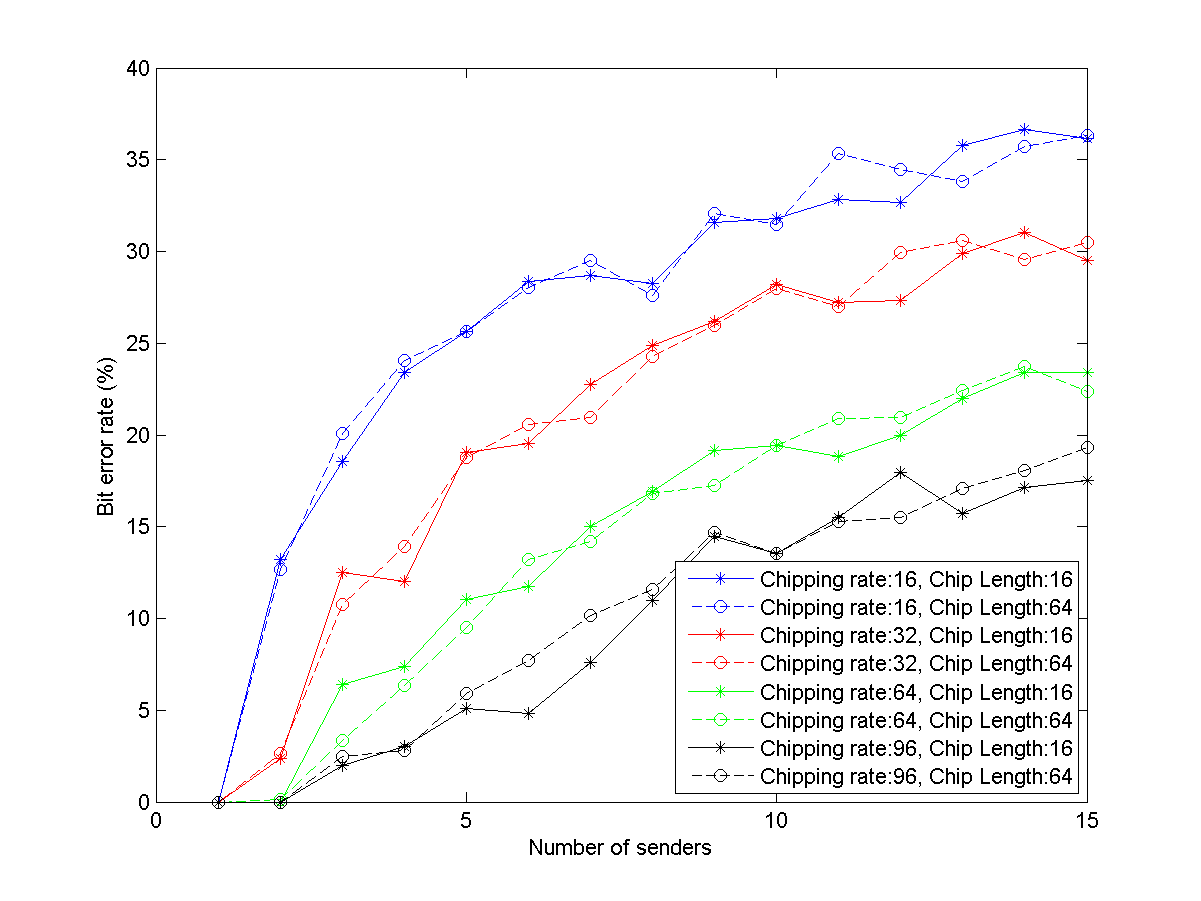
\includegraphics[width=0.5\textwidth]{imgs/results/plot_mode_dsss-test_numSenders-rep_20-dataRate_8-dataLength_128.png}
				\caption{DSSS: Multiuser}
				\label{fig:dsss_multiuser}
			\end{figure}
	
	\subsection{FHSS}
		
		Before going into the exact test cases, it is important to note that there is a problem with our implementation of fast frequency hopping, as it works badly with BPSK modulation. Various websites such as \cite{web-nl} emphasize the difficulty of using coherent data detection and that FSK is most often used. However, we followed our requirements and implemented BPSK.
		
		\subsubsection{Performance in presence of narrowband and wideband interference}~\\
			The results widely match expected behaviour, with performance deteriorating the more channels are jammed and wideband noise affecting all channels - and thus all configurations - equally.
			Importantly, we were not able to create configurations without crosstalk between the different channels, so this will have influenced all results.
			
			\begin{figure}[H]
				\centering
				\caption{}
				\begin{subfigure}[b]{0.5\textwidth}
					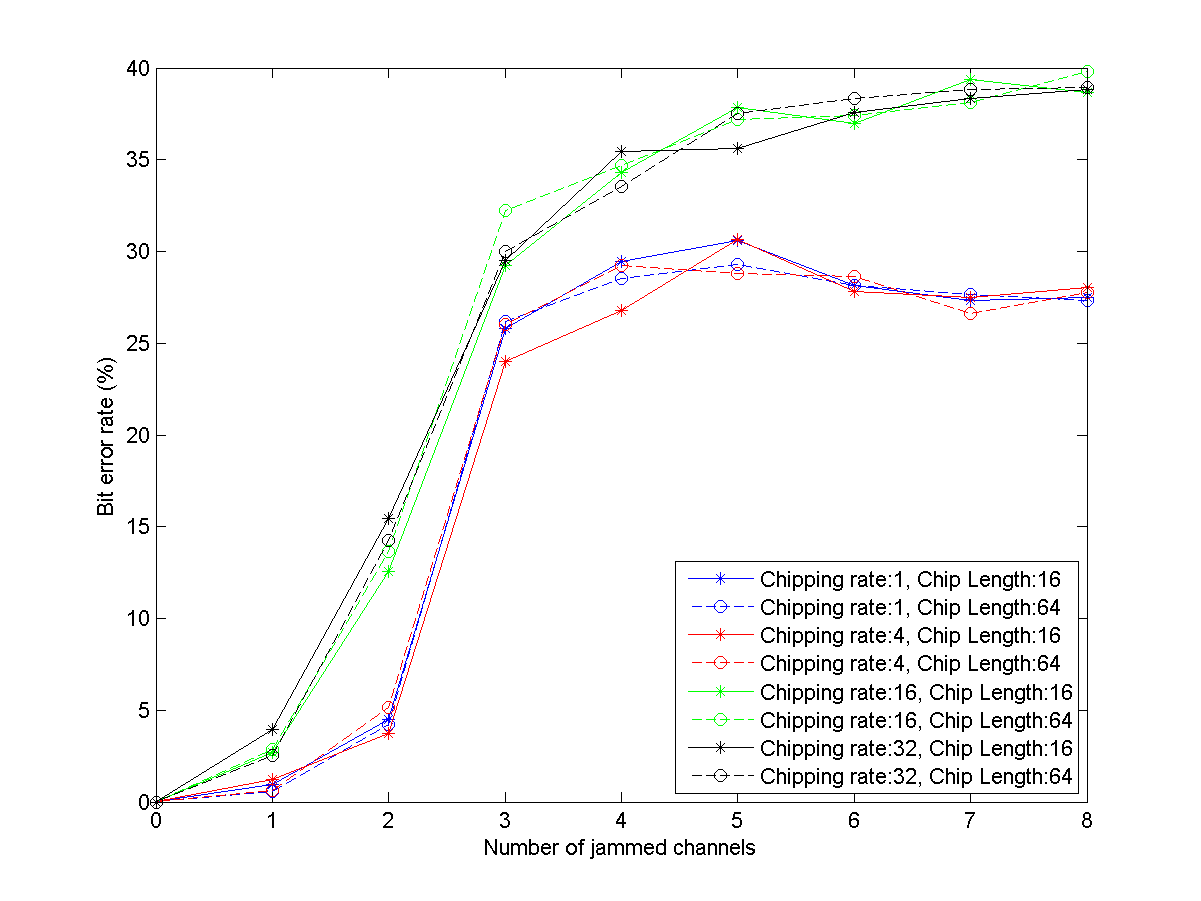
\includegraphics[width=\textwidth]{imgs/results/plot_mode_fhss-test_narrowband-rep_20-dataRate_8-dataLength_128.png}
					\caption{FHSS: Narrowband noise: $\Delta f= 64 \text{Hz}, p_f = 2.5$}
					\label{fig:fhss_narrowband}
				\end{subfigure}%
				~
				\begin{subfigure}[b]{0.5\textwidth}
					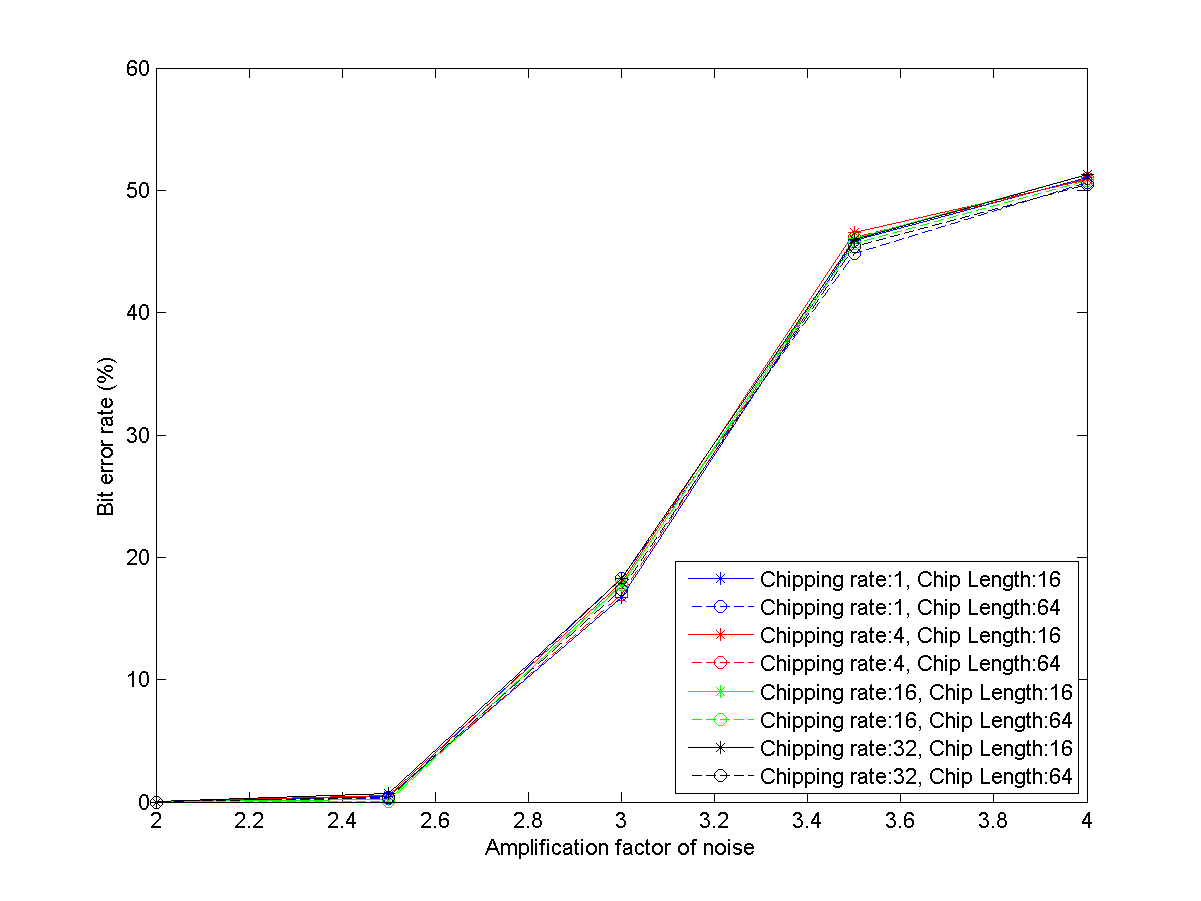
\includegraphics[width=\textwidth]{imgs/results/plot_mode_fhss-test_wideband-rep_20-dataRate_8-dataLength_128.png}
					\caption{FHSS: Wideband noise: $\Delta f= 200 \text{Hz}, f_{jam} = 550\text{Hz}$}
					\label{fig:fhss_wideband}
				\end{subfigure}
			\end{figure}
			
			
		\subsubsection{Performance with varying interference bandwidth and white Gaussian noise}~\\
			The results shown in Figure \ref{fig:fhss_bandwidth} again represent an estimation of performance under different - and presumably realistic - noise configurations.
			The results are similar to the ones from DSSS, with better performance under the influence of narrowband interference.
			Figure \ref{fig:fhss_gaussian} shows a more streamlined result than DSSS, which is caused by the bandwidths and channel configurations being invariable under the different parameter configurations.
	
			\begin{figure}[H]
				\centering
				\caption{}
				\begin{subfigure}[b]{0.5\textwidth}
					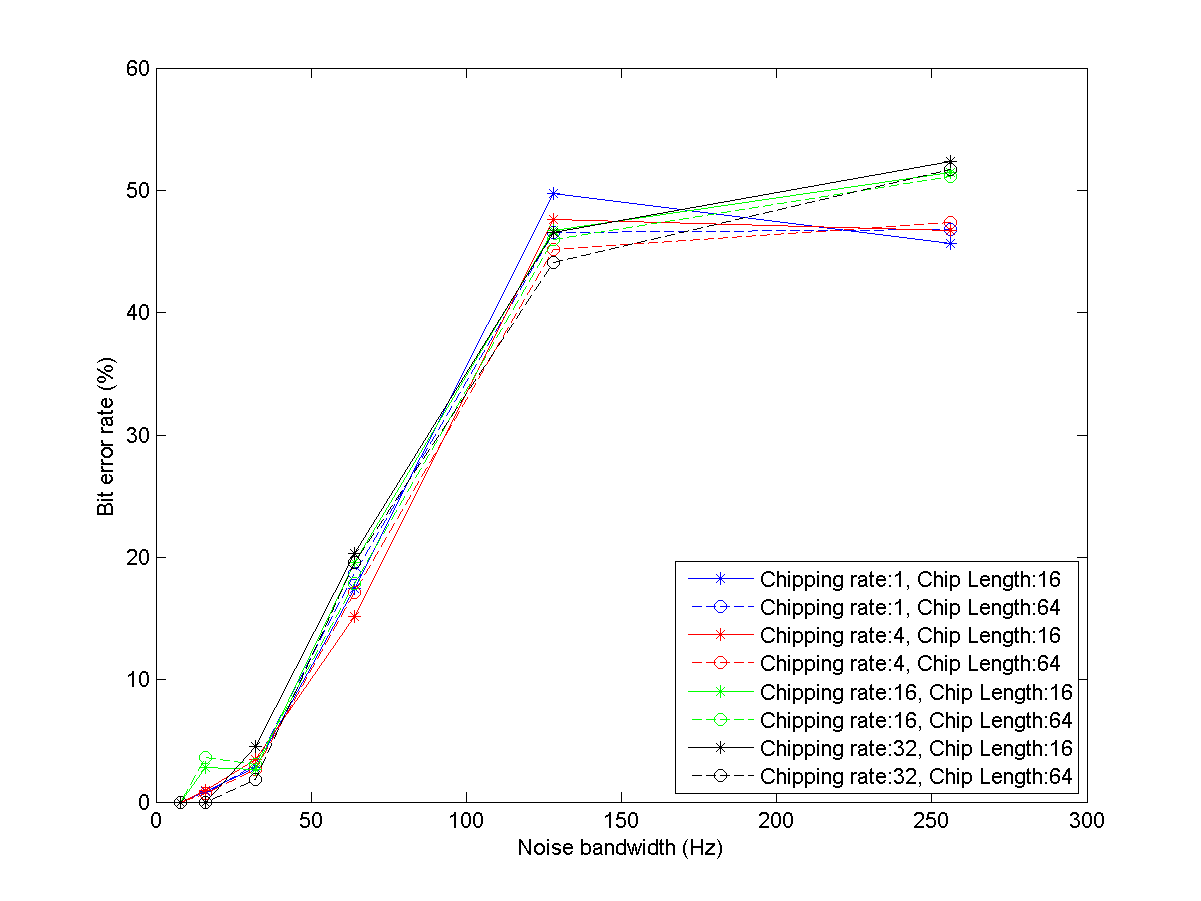
\includegraphics[width=\textwidth]{imgs/results/plot_mode_fhss-test_bandwidthAndPower-rep_20-dataRate_8-dataLength_128.png}
					\caption{FHSS: Various noise bandwidth and power: $p_f = (1,2,2.5,3,3.5,4)$}
					\label{fig:fhss_bandwidth}
				\end{subfigure}%
				~
				\begin{subfigure}[b]{0.5\textwidth}
					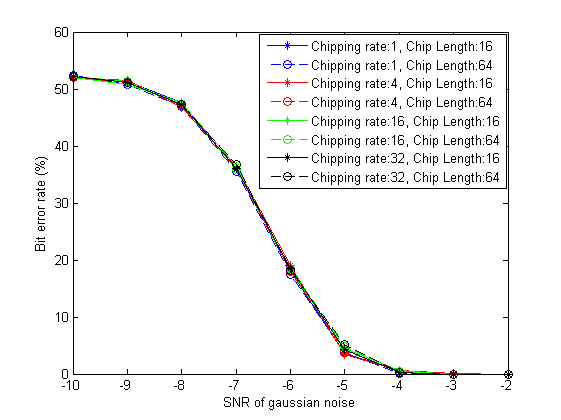
\includegraphics[width=\textwidth]{imgs/results/plot_mode_fhss-test_gaussianSNR-rep_20-dataRate_8-dataLength_128_fixedlegend.png}
					\caption{FHSS: Various SNR of white Gaussian Noise}
					\label{fig:fhss_gaussian}
				\end{subfigure}
			\end{figure}
		
		\subsubsection{Performance with multiple users}~\\
			The results shown match expected behaviour. The performance deteriorates quickly and bottoms at 40-50 \% BER when the number of users approaches the number of channels.
			
			\begin{figure}[H]
			\centering
				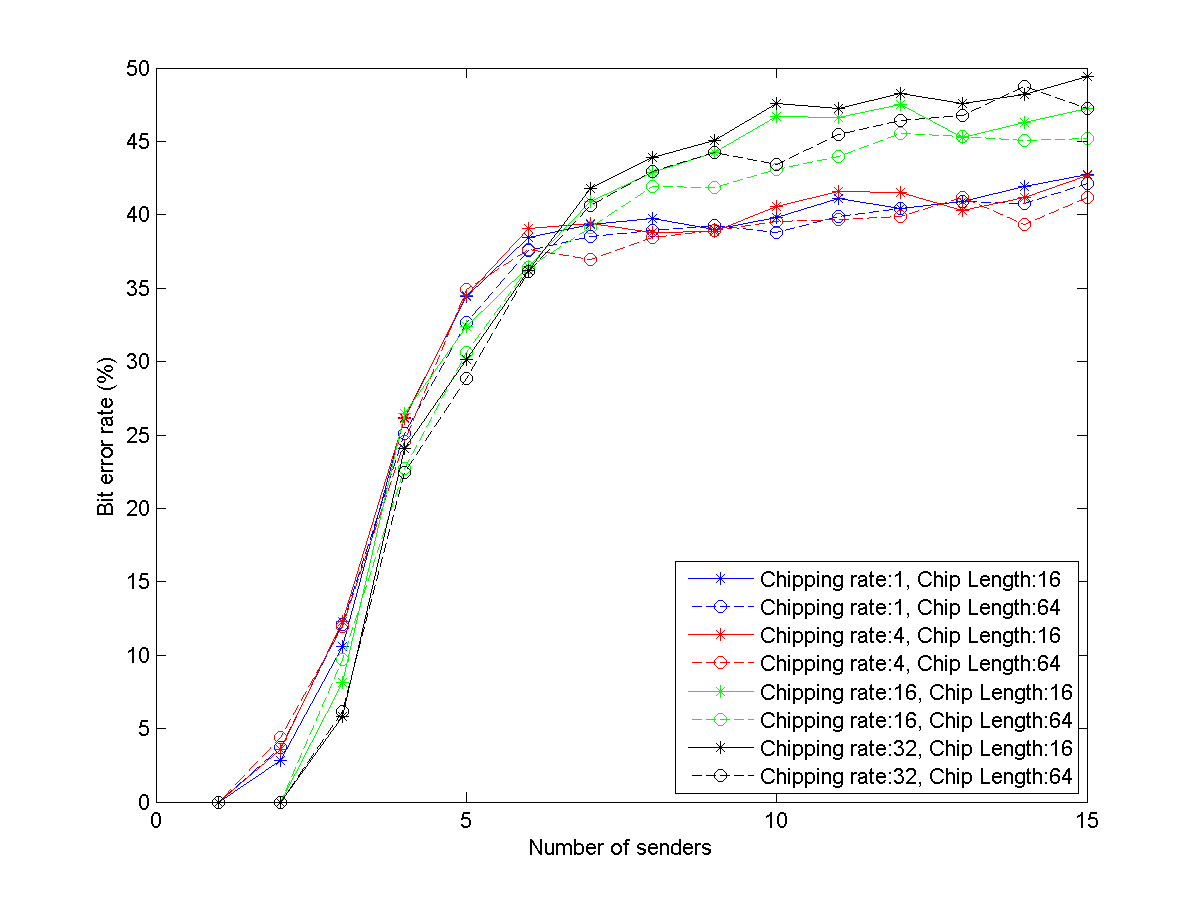
\includegraphics[width=0.5\textwidth]{imgs/results/plot_mode_fhss-test_numSenders-rep_20-dataRate_8-dataLength_128.png}
				\caption{Multiuser}
				\label{fig:fhss_multiuser}
			\end{figure}